\setlength{\parskip}{0.125in}

\chapter{The Announcement of the Competition}

The limited liability company ``Mail.Ru'', established and existing in accordance with the legislation of the Russian Federation 
and located at the address: 125167, Moscow, Leningradsky prospect, 39, building 79, hereinafter ``The Organizer of the Competition'',
invites individuals reached by the time of publication of this Announcement to 18 years, hereinafter ``Participant'',
to participate in the competition for the following conditions:

\section{The Name Of The Competition}

``Russian AI Cup’’.

The purposes of the Competition:
\begin{itemize}
\item increasing public interest to creation of software;
\item providing the Participants an opportunity to reveal their creative abilities;
\item the development of professional skills of Participants.
\end{itemize}

The Competition consists of 3 (three) stages, each of which ends with the determination of the Winners. The last stage of the Competition is decisive.

\section{Information about the Organizer of the Competition}

Name: The LLC ``Mail.Ru’’

The address of the location: 125167, Moscow, Leningradsky prospect, 39, building 79,

Postal address: 125167, Moscow, Leningradsky prospect, 39, building 79, Business Center ``SkyLight’’

Phone number: (495) 725-63-57

Website: http://www.russianaicup.ru

E-mail: russianaicup@corp.mail.ru

\section{The period of the Competition}

The Competition period: from 00.00 hours on 7 November 2016 to 24.00 hours 25 December 2016 Moscow time.

First week (from 00.00 hours on 7 November 2016 to 24.00 hours on 13 November 2016)
and fourth week (from 00.00 hours on November 28, 2016 to 24.00 hours 4 December 2016) of the Competition is testing.
During this period, the functionality of the website and judging system of the Competition may be incomplete,
and rules are subject to significant changes.

The timetable of the Competition:
\begin{itemize}
\item the first stage – from 00 hours 00 minutes on 26 November 2016 to 24 hours 00 minutes 27 November 2016;
\item the second stage – from 00 hours 00 minutes on 10 December 2016 to 24 hours 00 minutes 11 December 2016;
\item the third stage (final) – from 00 hours 00 minutes 17 December 2016 to 24 hours 00 minutes 18 December 2016.
\end{itemize}

\section{The conditions for obtaining the status of the Participant}

For participation in the Competition it is necessary to register in the System of the Organizer of the Competition.
This System are available on the website of the Organizer in the Internet at the following address: http://www.russianaicup.ru.

\section{The period of registration of Participants in the System of the Organizer}

Registration of Participants will be held from 00.00 hours on 7 November 2016 to 24.00 hours on 25 December 2016 inclusively.

\section{The territory of the Competition}

The Competition is held on the territory of the Russian Federation. Conducting all stages of the Competition is carried out
by remote access to the System of the Organizer via the Internet.

\section{The conditions of the Competition (the essence of the tasks, criteria and evaluation procedure}

The order of conducting of the Competition, the essence of the task, criteria and evaluation procedure specified in the
documentation in Chapter 2.

Documentation includes:
\begin{itemize}
\item The Announcement of the Competition;
\item The Agreement on organization and conducting of the Competition;
\item The Rules of the Competition;
\item Information data, which are contained in the System of the Organizer of the Competition.
\end{itemize}

The Participant can view the documents on the website of the Organizer in the Internet at the following address:
http://www.russianaicup.ru. Also the Participant can view the documents during the procedure of registration
in the System of the Organizer of the Competition.

The Organizer of the Competition has the right to change the documentation and conditions and to refuse to conduct
the Competition in accordance with the documentation and the provisions of the legislation of the Russian Federation.
In this case, the Organizer should notify the Participants about all changes by sending a notice,
in order and in the terms specified in the documentation.

\section{The procedure of determining the Winners and award Prizes. The prize Fund of the Competition}

Evaluation criteria of the Competition, the number and order of determining the Winners can be found in Chapter 2 of this document.

The prize Fund is formed at the expense of the Organizer of the Сompetition.

The prize Fund:
\begin{itemize}
\item 1st place --- Apple Macbook Pro 13\textquotedbl;
\item 2nd place --- Apple Macbook Air 13\textquotedbl;
\item 3rd place --- Apple iPad;
\item 4-6 places --- prizes;
\item 1-6 places in the Sandbox --- prizes.
\end{itemize}

All Participants who took part in the second or third stages, will be awarded a t-shirt. All Participants 
who took participation in the third stage, will also receive a hoodie with the logo of the competition.

All Participants, who will become winners, will be notified by sending a message to the email address,
indicated during the registration in the System of the Organizer.

Prizes will be sent out to Participants as packages by the Russian Post or by other postal service during two months after the end 
of the final stage. Terms of delivery of the prize to the postal address specified by the Participant depends on the terms of
delivery of the corresponding postal service. Postal addresses of the winners the Organizer receives from the credentials of Participant
in the System of the Organizer. The address must be specified by the Participant prize-winner during
three days after receipt of the notification about the prize.

In case of absence of a response in the designated period or failure to provide accurate data required for the delivery of prizes, the Organizer
has the right to refuse a Participant in the prize of the Competition. The cash equivalent of the prize is not provided.
 
The winners of the Competition must give the Organizer copies of all necessary documents for accounting and tax reporting. 
The list of documents which the Winner should give the Organizer, may include:
\begin{itemize}
\item a copy of the Winner’s passport;
\item a copy of the Winner’s certificate on statement on the tax account;
\item a copy of the Winner’s pension certificate;
\item information about the Bank account of the Winner;
\item Other documents that the Organizer will require of the Participant for the purposes of reporting on the conducted Competition.
\end{itemize}

Along with copies the Organizer of the Competition has the right to request the originals of the documents.

In accordance with subparagraph 4 of paragraph 1 of article 228 of the Tax Code of the Russian Federation, the Winner of the Competition who became the owner of the Prize, bear all costs
payment of all applicable taxes, stipulated by the legislation of the Russian Federation.

\section{The procedure and method of informing Participants}

Informing of Participants is carried out by placing the information on the Internet on the Website of the Organizer at the following address:
http://www.russianaicup.ru and also via the System of the Organizer of the Competition, during the period of Competition.

\chapter{About the world of CodeWizards 2016}

\section{General provisions of the game and the rules of the tournament}

This competition gives the opportunity to test your programming skills by creating artificial intelligence (strategy) to
control a wizard in a special game world (read more about the features of the world of CodeWizards 2016 in following sections).

Rules of the competition are based on the MOBA genre, which is popular in the world of computer games. In each game you will face five strategies of
others players. Also you will have four allies. Five strategies located on the same side are faction: Academy
or Renegades. The main goal of these five players is to destruct the base of the opposing faction.
The main personal goal of every wizard is to collect the highest possible number of score points.
The title of winner of the game, as well as all the other places are
distributed in accordance with the number of score points. Two or more players can share one place if their scores are equal. The player gets
points if his wizard damages, destroys or is just near in the time of death a of a unit of another faction. Also the player gets
points for some other actions. All players of the faction get a significant number of points in case of reaching the main team goal.

The rules of the game are nearly identical to the classical canons of the genre. Bases of factions are connected by three paths (top,
middle and bottom). Between these paths there are forests. The guardian towers are situated on the paths: $2$ towers of each faction
on each path. 
Thus, in the beginning of the game there are $14$ buildings on the map. With a certain time bases of each faction generate
$3$ similar squads of wizards’ minions: one for each path. They immediately run on their path in
the direction of the opposing faction base, attacking all enemies on their way.

The tournament is held in several stages, preceded by a qualification in the Sandbox.
Sandbox is a competition, which takes place during all period of the competition.
On each stage the player has a certain rating value.
It is an indicator of how well his strategy is playing in the games.

The initial value of the rating in the Sandbox is $1200$. At the end of any game this value can both increase and decrease. The victory
over the weak (low ranking) opponent gives a small increase, and the defeat of a strong opponent slightly reduces your
rating. Over the time, the rating in the Sandbox becomes more inert, thereby the influence of random long series of wins and
defeats by the place of the participant reduces.
However, it makes difficult to change the participant’s position with a substantial improvement of his strategy. To cancel
this effect, the participant may reset the variability of the rating to the starting value while submitting new strategy
(for this action it is necessary to activate the appropriate option).
If the new strategy is accepted by the system, participant's rating will be reduced by a significant amount after next game in the Sandbox. But
further participation in games will recover the rating quickly, and it will even become higher, if your strategy really became more effective.
It is not recommended to use this option for minor, incremental improvements of your strategy, as well as in cases when a new strategy is
insufficiently tested and the effect of changes in it is not known.

The initial value of the rating at each main stage of the tournament is $0$.
For each game participant gets a certain number of rating units, which depend on his place
(a system is similar to the system, which is  used in ``The FIA Formula One World Championship’’).
If two or more participants share same place, the total number of rating units for this place and for the following
$\texttt{number\_of\_such\_participants}-1$ places is divided
equally between these participants. For example, if two participants share the third place,
each receive half of the sum of rating units for third and fourth places. The result of the dividing is always rounded down.
Detailed information about the stages of the tournament will be provided in announcements on the project website.

Initially, all participants can only take part in Sandbox games. Players can send their strategies to the Sandbox, and
the last strategy accepted will be used by the system for qualification games. Each player takes part in about one qualification
game an hour. The judges can change this interval based on the capabilities of the testing system; however, for
most participants it will remain constant. There are a number of criteria that warrant the interval between qualification games
to be increased for a specific player. If the player has not sent a strategy in more than a week, the participation interval
for this specific player is doubled. Only the strategies accepted by the system count. For each <<crashed>> strategy in $10$ most recent
games in the Sandbox, an additional fine is accrued, which equals $20\%$ of the base testing interval. For more detail on the reasons why a strategy can be <<crashed>>
you can refer to subsequent sections.

Games in the Sandbox follow a set of rules that matches the rules of a random finished tournament stage or the rules for the next
(current) stage. The closer two players’ ratings are to each other in the Sandbox, the more likely they are to be in
the same game. The Sandbox starts before the first stage of the tournament and ends some time after the final stage (see the Schedule
of stages for detail). Additionally, the Sandbox is frozen while tournament stages are in progress. The results of games in the Sandbox
are used to select players for Round $1$, where $1080$ participants with the highest ratings are selected (if players have equal ratings, the priority is given
to the player who sends their final strategy version earlier), as well as additional players for subsequent stages of the tournament, including the Finals.

Tournament stages:
\begin{itemize}
 \item In \textbf{Round $1$} you will learn the rules of the game and basic controls of a Wizard. Each game in this stage
            will consist of $10$ players, who will be distributed into two factions, so that the difference between current
            ratings\footnote[1]{When a game is conducted as part of Round $1$, the ratings in this round are considered. When a game is conducted in the Sandbox using
            Round $1$ rules, the Sandbox ratings are considered.} of the participants in the two factions is minimum. The Wizard with the highest rating in each
            faction is appointed the Supreme Wizard. His strategy can send messages to other wizards from the same factions; it is also
            provided more computing resources (more CPU time). Functionality of the messages is limited, only allowing
            to send\footnote[2]{Regardless of the tournament stage, messages from the Supreme Wizard can be partially or fully
            ignored by other Wizards’ strategies.} other Wizards to a certain lane. In this mode, the Wizards can only use
            staff hit and <<Magic Missile>> spell, while the living energy of all structures is limited to half of
            the normal level. Damage ratio on accidental hit of a friendly Wizard equals $25\%$. Regardless of the stage
            of the championship friendly minions and structures take $0\%$ of damage. Round $1$, like all subsequent stages, consists of
            two parts, with a short break between them (the Sandbox is resumed during the break), which allows the players to improve their strategies.
            For games in each part, the latest strategy sent by a player before the beginning of that part is chosen by the system. Games are conducted in waves. In each
            wave, each player takes part in exactly one game. The number of waves in each part is determined by the testing system capacity, but it is
            guaranteed to be at least ten. $300$ participants with the highest ratings make it to Round $2$. For Round $2$,
            $60$ participants with the highest ratings in the Sandbox (as of the beginning of Round $2$), chosen from among those who didn’t make it to
            Round $1$.
 \item In \textbf{Round $2$} you will be improving your Wizard control skills and study the mechanics of the Wizard reaching
            new levels and learning new skills. The right approach to selecting and using skills is key to winning this stage.
            The way players are selected for the games is similar to Round $1$, but the Supreme Wizard has more skills this time. He can tell
            what skills other wizards in the factions should learn. Structures in this round have normal amount of living
            energy, and damage ratio on accidental hits of a friendly wizard equals $50\%$. To additionally complicate the task,
            after Round $1$ results are summarized, some of the weaker strategies will be discarded, so you will have to play against stronger
            opponents. At the end of Round $2$, the best $50$ strategies will make it to the Finals. $10$ participants will additionally be selected to the Finals, with
            the highest ratings in the Sandbox (as of the Finals starting), from among those who didn’t make it to the main tournament.
 \item \textbf{The Finals} is the most important stage in the tournament. After the first two stages, only the strongest players will remain. So in
            each game, you will be up against the strongest. Exactly. To manage five wizards in your faction,
            $5$ copies of your strategy will be running. Five wizards in the opposing faction will be controlled by $5$ copies of the
            opponent’s strategy. A random wizard is appointed the Supreme Wizard in each faction. He can control other wizards in that faction
            by sending messages in binary format. The restriction on binary data size is relatively high, but the message can only be received
            after a delay, which is proportional to its length. Damage ratio on accidental hit of a friendly wizard
            equals $100\%$. The winner is identified by adding up the points scored by all wizards in each faction. Otherwise
            the rules of the game are the same as in Round $2$. The Finals do have their peculiar features, however. The stage is still divided into
            two parts, but these no longer consist of waves. Each half of the Finals features games between all pairs of participants.
            The operation will be repeated if the time and capacity of the testing system allow.
\end{itemize}

After the Finals, all finalists are ranked according to their scores in descending order. In case of equal ratings, the participant whose
strategy for the Finals was sent earlier is ranked higher. Prizes for the Finals are awarded based on the place in the final
ranking. Top six finalists are awarded prizes:
\begin{itemize}
\item 1st place --- Apple Macbook Pro 13\textquotedbl;
\item 2nd place --- Apple Macbook Air 13\textquotedbl;
\item 3rd place --- Apple iPad;
\item 4-6 places --- valuable gifts.
\end{itemize}

After the Sandbox is over, all its participants, except for the Finals prize winners, are ranked according to their scores in descending order. In case of equal ratings, the participant
who sent the latest version of his/her earlier is ranked higher. Prizes for the Sandbox are awarded based
on the place in the final ranking. Top six players in the Sandbox are awarded valuable prizes.
 
\section{Description of the game world}
 
The game world is two-dimensional, and all units are round. The horizontal axis in this world is directed from left to right and vertical axis from top to bottom; the direction $0.0$ matches the horizontal axis direction, and positive rotation angle means clockwise rotation. Playing
area is a square with the upper left corner at ($0.0$, $0.0$), where each side length equals $4000.0$. No living
unit can leave the playing area.

\newpage
In the map layout below, copper color indicates the Academy buildings (larger circle means the faction base, smaller circles
indicate guardian towers), blue steel color indicates the Renegades’ structures, green means trees. $10$ color sports ($5$ in the lower left
corner of the map for Academy and $5$ in the upper right corner of the map for Renegades) indicate the Wizards’ spawning positions. It should be noted that
coordinates of the circle centers and tree radiuses in the forests can be different between games. New trees can also appear in the course of
the game.

The game engine transforms coordinates and directions before send it to the strategy of renegade wizard. So the strategy always ``think''
that it plays for the bottom left side, and the enemy is in the top right corner.

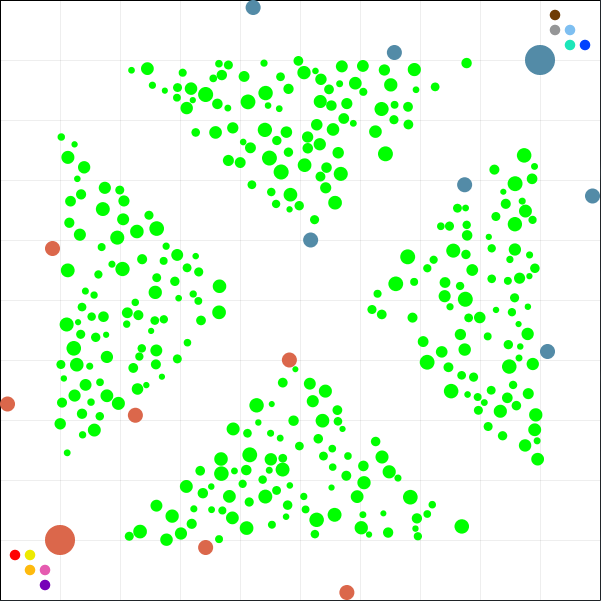
\includegraphics{images/map.png}

The time in the game is discrete, measured in <<ticks>>. At the beginning of each tick the game receives from the strategies the wizards’ desired actions in this tick
and updates the status of each wizard in accordance with these desires and the limitations of the game world. Next the game calculates changes in the world and the objects it
contains, which took place during the tick, and the process is repeated with the updated data. Maximum duration of any game equals $20000$ ticks, but the game
can be terminated early if either faction has reached its team goal, or all participants strategies have been <<crashed>>. It is extremely
unlikely, but not impossible, that both factions will reach their team goals in the same tick. Then additional points
are awarded to all game participants.

<<Crashed>> strategy is not able to control a wizard anymore. The strategy is considered <<crashed>> in following cases: 
\begin{itemize}
  \item The process of the strategy unexpectedly exited, or there was a problem with communication protocol between the strategy and a game server. 
  \item The strategy exceed one of the time limits.
For one tick the strategy has $5$ seconds of real time. For all the game the strategy process usually has
        \begin{equation}
        20\times\textit{<game\_duration\_in\_ticks>}+5000
        \end{equation}
        milliseconds of wall time and
        \begin{equation}
        10\times\textit{<game\_duration\_in\_ticks>}+5000
        \end{equation}
        milliseconds of processor time. The master wizard strategy has
        \begin{equation}
        30\times\textit{<game\_duration\_in\_ticks>}+5000
        \end{equation}
        milliseconds of wall time and
        \begin{equation}
        20\times\textit{<game\_duration\_in\_ticks>}+5000
        \end{equation}
        milliseconds of processor time.\footnote[3]{Despite the limit for the wall time is notably higher, than limit for the processor time,
        artificial <<slowdowning>> of strategy with commands like <<\texttt{sleep}>> is prohibited (any  other attempts to slowdown/destabilize
        the system are prohibited too. In case of such behavior, the jury can disqualify user from the competition and block his account.}
        Time formula includes max game duration. This limit covers as a user code time as a client-server communication time.
        The time limit remain a constant even if the real game time is different.
  \item The strategy exceeded a memory limit. Strategy process can not use more than 256 MB of RAM at the same time.
\end{itemize}

Discovering units on the map is limited by the fog of war. The strategy takes the information only about the units,
locating in vision range \footnote[4]{The distance between the units is the distance between their geometric centers.}
of the wizard or any unit from his fraction.

\section{Unit classes}

There are $6$ classes of units in the CodeWizards 2016 world, some of which are then divided into types:
\begin{itemize}
            \item wizards;
            \item projectiles: Magic Missile (\texttt{MAGIC\_MISSILE}), Frost Bolt (\texttt{FROST\_BOLT}), Fireball (\texttt{FIREBALL}) and
            Dart (\texttt{DART});
            \item bonuses: Empower (\texttt{EMPOWER}), Haste (\texttt{HASTE}) and Shield (\texttt{SHIELD});
            \item structures: Faction Base (\texttt{FACTION\_BASE}) and Guardian Tower (\texttt{GUARDIAN\_TOWER});
            \item minions: Orc-woodcutter (\texttt{ORC\_WOODCUTTER}) and Fetish Blowdart (\texttt{FETISH\_BLOWDART});
            \item trees.
\end{itemize}
 
Wizards, structures, minions and trees are living units. The main characteristics of every living unit are their current and
maximum amount of living energy. Generally, when living energy drops to zero, a unit is considered dead and
is removed from the game world. Wizards are the only living units that feature health regeneration. Each tick, they automatically
recover some of their living energy. Regeneration rate is a real number, usually less than one.
Over several ticks it may look like a wizard is not regenerating health, but that is not true. Total regeneration over
several ticks is stored in a special pool. A wizard is considered dead if the integer part of his living energy drops to
zero, regardless of how much energy is currently stored in the pool.
 
Comparative characteristics of the living units are shown in the table below:

\begin{tabular}{| l | l | l | l | l | l | l |}
            \hline
            Living unit characteristics            & Wizard                & Orc   & Fetish & Guardian Tower         & Faction Base           & Tree    \\
            \hline
            Radius                                 & $35$                  & $25$  & $25$   & $50$                   & $100$                  & $20-50$ \\
            Max life                               & $100$\footnotemark[5] & $100$ & $100$  & $1000$\footnotemark[6] & $2000$\footnotemark[6] & $6-36$  \\
            Vision range                           & $600$                 & $400$ & $400$  & $600$                  & $800$                  & ---     \\
            Ranged attack distance\footnotemark[7] & $500$                 & ---   & $300$  & $600$                  & $800$                  & ---     \\
            Melee attack distance\footnotemark[8]  & $70$                  & $50$  & ---    & ---                    & ---                    & ---     \\
            Attack cooldown                        & $30$\footnotemark[9]  & $60$  & $30$   & $240$                  & $240$                  & ---     \\
            Attack damage                          & $12$\footnotemark[10] & $12$  & $6$    & $36$                   & $48$                   & ---     \\
            \hline
\end{tabular}
 
\footnotetext[5]{Maximum living energy for a zero-level wizard. Maximum energy is increased by $10$ for each level achieved.}
\footnotetext[6]{Actual living energy of a structure at a specific stage of the tournament can be different from the value shown in the table.}
\footnotetext[7]{Maximum duration of a projectile flight or maximum distance between unit centers.}
\footnotetext[8]{Maximum possible distance to the nearest point of the target.}
\footnotetext[9]{Minimum possible interval between a wizard’s two consecutive attacks or spells. Each action type
            has its own limited interval.}
\footnotetext[10]{Base damage from a close-combat attack or the simplest spell, <<Magic Missile>>. The damage can be increased by the wizard
            learning certain skills.}
 
A bonus has a radius of $20$, regardless of the bonus type.
 
Comparative characteristics of the projectiles are shown in the table below:
 
\begin{tabular}{| l | l | l | l | l |}
 \hline
 Projectile characteristics     & Magic Missile & Frost Bolt & Fireball         & Dart \\
 \hline
 Radius         & $10$          & $15$          & $20$                      & $5$  \\
 Speed                      & $40$          & $35$          & $30$                      & $50$   \\
 Damage on direct hit & $12$            & $24$          & $24$\footnotemark[11] & $6$       \\
 \hline
\end{tabular}
 
\footnotetext[11]{Formally, a fireball does not inflict any damage on direct hit, but as it explodes on impact, it causes damage to all
            living units within the distance of $100$ between the center of the fireball and the nearest point of the living unit, including the unit that
            was directly hit. If said distance does not exceed the fireball radius, the explosion causes maximum damage. As
            distance increases, the damage is reduced in a linear manner, until it reaches half of the value in the table at the periphery of the explosion radius.}
 
In addition to causing damage, the frost bolt also freezes (\texttt{FROZEN}) the target for $60$ ticks. The frozen unit cannot
move or perform any actions, but the number of ticks remaining until the next action can be applied keeps counting down.
Buildings and trees cannot be frozen. A wizard’s strategy does not gain control until the freezing period is over.
 
The fireball explodes when it hits the target or reaches maximum flight distance, causing damage to all living units within
the distance of $100$ between the center of the fireball and the closest point of the unit. All units receiving damage from the explosion also
get the burning status (\texttt{BURNING}). It remains in effect for $240$ ticks, causing $24$ units of damage over this time. Damage from several
statuses of the same type is accumulated.
 
A building attack does not create a projectile. Damage is caused instantly due to a magic blast.

The second Guardian Tower on the lane is immune to damage if the first tower is alive. To be able to attack the opposite Faction Base the
wizards should destroy both enemy towers on any lane.

\section{Wizard characteristics}
 
The main characteristics of every living unit are current and maximum amount of living energy. However, a wizard also has several
other important characteristics. For example, the wizard’s ability to cast spells is limited by current and maximum amount
of magic energy and its regeneration rate.
 
Unlike other living units, a wizard cannot be killed; you can only destroy his physical shell. After some
time the wizard will respawn in a new body. Respawn can occur at least $1200$ ticks after the wizard’s death and at least $2400$ ticks since
his last respawn. The wizard respawns at his respawn position, or next to it if the position is currently occupied.
 
In some game modes, the wizard can accumulate experience and increase its level. Every wizard starts with zero level and
grows to the maximum level of $25$. Nevertheless, the rules of the game are balanced so that achieving level $15$ is almost impossible.
The wizard gets experience in the same amount and on the same occasions as when the player controlling him gets points, unless
the wizard is dead and awaits respawn at that tick. A wizard needs to score $50$ experience points to get to level one; an additional $100$ points
for level two, $150$ for level three, $200$ for level four, and so on.
 
The amount of living energy at level zero equals the amount of magic energy and equals $100$ points. Both types of energy grow
$10$ points each level. Living energy regenerates at $0.05$ ticks$^{-1}$ at level zero, and increases
by $0.005$ ticks$^{-1}$ with each level. The respective characteristics of magic energy are $4$ times higher.
 
A wizard can learn exactly one skill with each level achieved. Skills are divided into $5$ groups. The skills within each group
are ordered and can be learned only in sequence. The number of skills in each group equals $5$. The first and the third skill in each group, as
a rule, increase one of the wizard’s characteristics. The second and fourth one are auras. An aura operates similarly to a
passive skill, but is applied not just to the wizard himself, but also to all friendly wizards within the distance of
$500$ or less. If several auras apply to a wizard that improve one and the same quality of the unit, only
the one with the biggest effect is taken into account. The final, fifth skill in each group is the most important (<<ultimate>>) skill. It
enables the wizard to cast a new spell or substantially improves an existing spell.

\begin{itemize}
            \item Passive skills and auras in the first group increase the distance of the wizard’s spells by $25$ for each level. Thus, a wizard
            who has mastered all these skills will be able to cast spells at the distance of $600$. Additionally, all friendly wizards nearby will get
            extra distance of $50$ for their spells. The last skill in this group allows using the <<Magic Missile>> spell
            without a delay. By default, the delay in casting this spell is $60$ ticks. Nevertheless, the overall delay on a wizard’s
            actions still applies.
            \item Passive skills and auras in the second group increase the damage caused by magic projectiles by $1$ for each level. The last skill
            in this group allows the wizard to use the <<Frost Bolt>> spell, which causes substantial damage to a single opponent, in addition to
            freezing him for $60$ ticks.
            \item Passive skills and auras in the third group increase the damage caused by staff hit in close combat by $3$ for each level. The last
            skill in this group allows the wizard to cast the <<Fireball>> spell, which causes damage to a group of opponents, in addition to
            setting them on fire.
            \item Passive skills and auras in the fourth group increase the wizard’s maximum possible movement distance in one tick by $5\%$ for each level.
            The total increase from the four skills is $20\%$, while aura adds $10\%$ movement to friendly wizards
            nearby. The last skill in this group enables the wizard to use the <<Haste>> spell, which gives a friendly
            wizard the \texttt{HASTENED} status for $600$ ticks. This status adds an extra $30\%$ to the unit’s movement speed, in addition to
            increasing the turning speed by $50\%$. Several statuses of the same type are not accumulated.
            \item Passive skills and auras in the fifth group decrease the damage received from magic projectiles and structure attacks by $1$ for each level.
            The last skill in this group allows the wizard to cast the <<Shield>> spell, which gives a friendly wizard the
            \texttt{SHIELDED} status for $600$ ticks. This status reduces any direct damage by $25\%$. The only exception is the damage from
            \texttt{BURNING} status. Several statuses of the same type are not accumulated.
\end{itemize}
 
You can find the full list of available skills in the documentation to enumeration \texttt{SkillType} (Chapter 4).
 
\section{Control of the wizard}
 
In the beginning of each tick, the game simulator sends data about the current state of the part of the world, visible to the wizard,
to the strategies of each alive wizard. In response the strategy sends a set of instructions for control of the wizard, encapsulated in the object of the \texttt{Move} class.
 
These instructions are processed in the following order:
\begin{itemize}
            \item Each wizard learns the skill \texttt{move.skillToLearn}, if it is set. The game simulator will ignore the instruction,
            if the number of skills learned by the wizard is already equal to his level or if the wizard has not yet learned all the previous skills in the group.
            \item Then wizards randomly perform actions, set in \texttt{move.action}:
            \begin{itemize}
            \item \texttt{NONE}. \textit{Don't do anything.}
            \item \texttt{STAFF}. \textit{Strike with the staff.} The attack will strike all living units which centers are in the sector of $-\pi / 12$ to $\pi / 12$.
                    The distance from the center of the wizard to the nearest target point must not exceed $70$. If the wizard died in the result
                    of the staff strike of another wizard, made earlier within the same tick, then the staff strike will still be performed. The dead
                    wizard will not gain experience for the caused damage, nevertheless, the player whose strategy controls this wizard, will receive
                    a relevant amount of points.
            \item \texttt{MAGIC\_MISSILE}, \texttt{FROST\_BOLT} or \texttt{FIREBALL}. \textit{Create the relevant magic projectile.}
                    When creating a projectile, its center is set equal to the center of the wizard, and its direction is determined as
                    \texttt{wizard.angle + move.castAngle}. Value \texttt{move.castAngle} is set by the strategy and is limited
                    by the interval from $-\pi / 12$ to $\pi / 12$. Additional parameters \texttt{move.minCastDistance} and
                    \texttt{move.maxCastDistance} determine the minimum and the maximum distance of the projectile cast. If the distance from the center
                    of the projectile to the point of its appearance is less than \texttt{move.minCastDistance}, then the projectile will pass through all
                    other game objects, except for trees. If the distance from the center of the projectile to the point of its appearance is more than
                    \texttt{move.maxCastDistance}, then the missile will be removed from the game world. At that moment, the projectile of the \texttt{FIREBALL} type will explode.
                    Collisions of the magic projectile with the wizard, who created it, are ignored. If the wizard died in the result of the staff strike
                    of another wizard, made earlier in the same tick, then the missile will not be created.
            \item \texttt{HASTE} or \texttt{SHIELD}. \textit{Apply relevant magic status to the target.} The status is applied to
                    a friendly wizard with identifier \texttt{move.statusTargetId} or to the wizard himself if such a wizard is not
                    found. The target must be located in the sector from $-\pi / 12$ to $\pi / 12$, and the distance to it must not exceed
                    \texttt{wizard.castRange}. Value \texttt{wizard.castRange} for a wizard of the zero level is equal to $500$, but it may
                    grow to $600$ after some skills are learned. If the wizard died in the result of the staff strike of another wizard,
                    made earlier within the same tick, the status will not be applied.
            \end{itemize}
 
            There must be not less than $30$ ticks between any two consecutive acts of the wizard, different from \texttt{NONE}. For each
            act there is its own delay, which limits consecutive use of two actions of one
            type. Creation of a missile or application of the status consumes magic energy of the wizard. Desired action will be ignored
            if there is not enough energy.
 
            \begin{tabular}{| l | l | l | l |}
            \hline
            Characteristics of the act & Staff strike & Acceleration & Shield   \\
            \hline
            Cooldown           & $60$          & $120$         & $120$ \\
            Manacost               & ---               & $48$          & $48$  \\
            \hline
            \end{tabular}
 
            \begin{tabular}{| l | l | l | l |}
            \hline
            Characteristics of the act & Magic Missile    & Frost Bolt & Fireball \\
            \hline
            Cooldown           & $60$\footnotemark[12] & $90$                  & $120$         \\
            Manacost               & $12$                      & $36$          & $48$          \\
            \hline
            \end{tabular}
            \item Then wizards are again randomly put in order and they are moved.
 
            In the CodeWizards world, 2016 there is no inertia, and the change of speed happens instantaneously. Strategy request \texttt{move.speed} determines
            the move of the wizard forward/back, and \texttt{move.strafeSpeed} --- sideways movement. Value \texttt{move.speed} is limited
            by the interval from $-3.0$ to $4.0$, where positive values mean the forward movement, and negative --- backward movement. Value
            \texttt{move.strafeSpeed} is limited by the interval from $-3.0$ to $3.0$, where positive values mean the right side
            movement, and negative values --- left side movement. Limits of both intervals may be extended depending on the skills learned by the wizard, depending
            on the influence of some auras, as well as in case of application of the \texttt{HASTENED} status. Both types of movement may be performed
            simultaneously within one tick, but in that case an additional limitation will be applied: if value
            \texttt{$\sqrt{(\frac{move.speed}{maxSpeed})^2 + (\frac{move.strafeSpeed}{maxStrafeSpeed})^2}$} is more than $1.0$, then both settings
            of the movement speed (\texttt{move.speed} and \texttt{move.strafeSpeed}) will be divided by this value by the game simulator.
            \texttt{maxSpeed} and \texttt{maxStrafeSpeed} --- relevant limitations, applied to the movement of the wizard this tick (with
            consideration of the direction of the movement, learned skills and affecting auras and statuses).
 
            Movement of wizards is performed sequentially, according to the selected order. At that, partial movement of the wizard is not
            applied. If it is impossible to change the location of the wizard for the whole value of the movement, set by the strategy\footnotemark[13], then
            his movement is postponed. After the iteration is completed, the game simulator again iterates all the wizards and attempts
            to relocate those, whose position has not yet changed within this tick, This happens until all the wizards have been relocated.
            If in the course of the next iteration none of the wizards was moved, then the operation will be terminated.
 
    \item All wizards turn for the angle set by the strategy. By default the absolute angle change can not be higher than $\pi / 30$.
          Hastened wizard turns $1.5$ times faster.
\end{itemize}
 
\footnotetext[12]{Delay in the application of the spell <<Magic Missile>> may be less in the result of learning of some skills.}
\footnotetext[13]{After the relocation a wizard is partially or completely beyond the limits of the map or crosses some other
            alive unit.}
 
Apart from the listed actions, the supreme wizard can send messages to other wizards from his faction. Field
\texttt{message.lane} contains a recommendation to go to the relevant path. Field \texttt{message.skillToLearn} becomes available
in Round $2$ and contains a recommendation to learn the specified skills. A skill may require learning of other preliminary skills or may be
unavailable due to the low level of the wizard. The wizard is recommended to memorize the task and move towards
its implementation. At that, a later task has a higher priority. In the Finals the supreme wizard has
the opportunity to send text messages. Field \texttt{message.rawMessage} is a byte array, its maximum length is
$1024$. Usually wizards receive messages in the next tick after the dispatch, but if there is a text part, the receipt
will be delayed for \texttt{ceil(message.rawMessage.length / 2.0)} game ticks. If there is a registered message in the system for one of the
wizards, but it has not yet been received by him, then new messages to this wizard will be ignored.
 
\section{Other game objects}
 
Each $750$ ticks the base of each faction generates $3$ troops of minions: per one for each of the lanes. Each troop consists of three orks
and one fetish. The troop directly rushes down its path in the direction of the base of the opposite faction, attacking all enemies on its way.
Wizards use minions as the cannon fodder. At that, they are trying to stay in the safe area and attack the enemy from
the distance.
 
In the forest area neutral minions may appear with some probability. Usually they are not aggressive, but if one of the minions is damaged,
all the neutral minions in the area will rush to the offender, attacking anyone on their way.

A minion can move strictly forward not faster than $3$ ticks$^{-1}$. The absolute angle change of a minion can not be higher than $\pi / 30$.
 
Every $2500$ ticks up to two bonuses may appear on the map. The bonuses are created at the two following points: $(1200, 1200)$ and
$(2800, 2800)$. If any part of the new bonus area is already occupied by a wizard or by an existing bonus, then the creation of the bonus
will be postponed till the end of the next interval.
 
\section{Collision of units}

\begin{itemize}
 \item Collision of alive units between them as well as with the borders of the map is not allowed by the game simulator.
 \item If the distance from the center of an alive unit to the center of the projectile is less than or equal to the sum of their radii, then the alive unit will be damaged, and the projectile
            will be removed from the game world. At that, the fireball explodes and damages all alive units in the area.
 \item If the distance from the center of a wizard to the center of the bonus is less than or equal to the sum of their radii, then the wizard receives a magic status
            for $2400$ ticks, depending on the bonus type:
            \begin{itemize}
            \item \texttt{EMPOWER} increases the damage caused by a wizard in the result of the staff strike and in case of hitting the target
                    with the magic projectile by $2$.
            \item \texttt{HASTE} speeds up the movement of a wizard similar to the cognominal spell.
            \item \texttt{SHIELD} decreases the damage, received by a wizard, similar to the cognominal spell.
            \end{itemize}
\end{itemize}
 
All types of collisions not described in this document are ignored by the game simulator.
 
\section{Scoring}
 
The wizard receives experience in the same amount and in the same cases, when the player, controlling the wizard, receives points, except for when
the wizard is dead in the tick when points are scored and is waiting for respawn. Points are given for the following actions:
\begin{itemize}
            \item Causing damage to buildings and wizards of the opposing faction. Damages are accounted with a coefficient of $0.25$. Rounding
            is done down to the nearest integer. Points for damages are given only to the player, whose wizard caused these
            damages.
            \item Destruction of buildings or wizards of the opposing faction, as well as minions of any faction, different from the wizard's faction.
            Total reward for buildings and minions is $25\%$ of the maximum amount of their life energy, for wizards ---
            $100\%$. Destruction may be done by the wizard himself or by any other unit from his faction. Experience is equally
            distributed among all friendly wizards, the distance to whom from the target does not exceed $600$. At that, if the number of
            such wizards is more than one, then the total reward increases by $67\%$. Rounding is done down to the nearest
            integer.
            \item Collection of any bonus gives $200$ score/experience points.
            \item In case of destruction of the opposing faction base, all friendly players receive $1000$ points. The game is finished in this case.
\end{itemize}
 
\chapter{Creation of the strategy}
 
\section{Technical part}
 
To create a strategy, first you need to do is to choose one of the supported programming languages\footnote[14]{For all programming languages
32-bit compiler/evaluator versions are used.}: Java (Oracle JDK 8), C\# (Roslyn 1.3+), C++14 (GNU MinGW C++
6.2+), Python 2 (Python 2.7+), Python 3 (Python 3.5+), Pascal (Free Pascal 3.0+), Ruby (JRuby 9.1+, Oracle JDK 8). Possibly this set
will be extended. On the project website you can download the user pack for each of the languages. It is allowed to modify only one
file in the pack, which is meant for maintenance of your strategy, for example MyStrategy.java (for Java) or MyStrategy.py (for
Python)\footnote[15]{C++ is the exception, because for it, it is possible to modify two files: MyStrategy.cpp and MyStrategy.h. At that, the presence
in the archive of the MyStrategy.cpp file is mandatory (otherwise the strategy cannot be compiled), and the presence of the MyStrategy.h file --- optional. In case
of its absence a standard file from the pack will be used.}. All other files of the pack in the course of compilation of the strategy will be replaced
with standard versions. Nevertheless, you can add your own files with code to the strategy. These files must be placed in the same directory, as the
main strategy file. When submitting the solution, all of them must be placed into one ZIP-archive (all of them must be located in the archive root). If
you do not add new files in the pack, it is enough to send the strategy file (via the dialog when selecting the file) or input its code into
the text field.
 
After you sent your strategy, it is put in queue for testing. First, the system will try to compile a submission with your
files, and then in case of success, it will create several short (of $200$ ticks) games of different formats\footnote[16]{Main
parameters of the game format are the number of players participating in the game, and the number of units under control of each player.
In a short form, the format is written as $\texttt{<number\_players>}~\times~\texttt{<number\_units>}$, for example, the string $4\times3$ means
that the game has a format with $4$ players, and each controls three units. The format may be complimented with the clarification, if
the short notation of formats for different stages of the championship is the same. Pay attention, that in the Final games of this championship, each wizard of
one faction is controlled by the participant's strategy launched as a separate process. From the point of view of the game API, these wizards
will be virtually distributed among five different players, but determination of the winner will only depend on the sum of their points, and not on
distribution to specific wizards.}: $10\times1$, $10\times1$ with unlocked skills of wizards and $2\times5$. In order to control
the wizard of each of the participants of these games, a separate process with your strategy will be launched, and for this strategy
to be considered accepted (correct), none of the copies of the strategy may <<crash>>. The players in the test games will be assigned names in the
format <<\texttt{<name of\_player>}>>, <<\texttt{<name of\_player> (2)}>>, <<\texttt{<name of\_player> (3)}>> and etc.
 
After the successful completion of the described process, your submission receives the status <<Accepted>>. The first successful submission means also your
your registration in the Sandbox. You are assigned the start rating ($1200$), and your strategy starts participating in periodic
qualification games (see the description of the Sandbox for more details). Also the function to create
your own games becomes available, in which you can choose the strategy of any player as opponent (including your own), created before
the moment of your last successful submission. The games created by you do not affect your rating.
 
The system has limitations in relation to the number of submissions and user games, specifically:
\vspace{-0.15in}
\begin{itemize}
 \item It is forbidden to send strategies more often than three times per five minutes.
\vspace{-0.10in}
 \item You cannot create more than two user games in five minutes.
\vspace{-0.10in}
\end{itemize}
 
In order to simplify the adjustment of small changes in the strategy, the system has the possibility to perform a test submission (flag <<Test submission>>
in the strategy submission form). The test submission will not be displayed to other users, does not participate in the qualification games in the Sandbox and
games of the tournament stages, also it is impossible to create games with it by oneself. Nevertheless, after the system accepts this submission, the system
will automatically add the test game with ten participants (format$10\times1$): the test submission itself and nine strategies from
the <<Quick start>> section. The test game will be visible only to the participant, who created this test submission. The base duration of this test
game is $2000$ ticks. The dispatch of test games is limited in the same way as the dispatch of normal submissions. Test games do not influence
the frequency of games creation by the user.
 
The players have a possibility to view past games in the special visualizer. To do that it is necessary to press the <<View>> button in the list of games
or press the <<View game>> button on the page of the game.
 
If you watch the game with participation of your strategy and noticed something strange in its behavior, or your strategy does not do what you
expect from it, you can use a special utility Repeater to perform a local repeat of the game. The local repeat of the
game --- is the opportunity to launch the strategy on your computer in such a way, that it sees the game world around the same way, as it was on
the server while testing. This will help you to perform adjustments, add logging and watch the reaction of your strategy during each game
moment. To do that, download Repeater from the CodeWizards 2016 website (section <<Documents>> $\rightarrow$ <<Repeater Utility>>) and unzip it.
To launch Repeater, you need installed software Java $8+$ Runtime Environment. Pay attention, that any cooperation of your
strategy with the game world during the local repeat is completely ignored. This means, that at each moment of time the surrounding world
looks exactly the same for the strategy, as it looked during the game in the course of testing on the server, and does not depend on the actions your strategy
performs. The Repeater utility only posses the data, which were sent by your strategy, but does not posses the complete recording of the game. Thus
the visualization of the game is not possible. You can read more information about the Repeater utility in the relevant section on the website.
 
Apart from everything mentioned above, the players have an opportunity to launch simple test games locally on their computer. To do that,
it is necessary to download a zip-file with the Local runner utility from the website section <<Documents>> $\rightarrow$ <<Local runner>>. Use of this
utility will allow you to test your strategy in conditions, similar to the conditions of the test game on the website, but without any limitations in relation to the
number of created games. Renderer for local games is significantly different from the renderer on the site. All game objects in it are displayed
schematically (without colorful models). It is very easy to create a local test game: launch Local runner with the help of
the relevant launch script (*.bat for Windows or *.sh for *nix systems), then launch your strategy from the development area (or any way
that is convenient for you) and watch the game. During local games, you can make adjustments to your strategy, put break points.
But remember, that Local runner waits for the strategy response for not more than $30$ minutes. Upon expiry of this time, it will consider
the strategy <<crashed>> and will continue to work without it.
 
\section{Control of the wizard}
 
In the beginning of the game an object of the \texttt{MyStrategy} class will be created for your wizard, and in the field of this object the strategy can save information
about the course of the game. Control of the wizard is performed via the \texttt{move} method of the strategy, which is called once per tick. The method
receives the following parameters:
\begin{itemize}
 \item the wizard \texttt{self}, for which the method is called;
 \item current state of the world \texttt{world};
 \item set of game constants \texttt{game};
 \item object \texttt{move}, by setting the parameters of which the strategy determines the behavior of the wizard.
\end{itemize}
 
Implementation of the user shell of the strategy in different languages may differ, nevertheless, in the general case it is \textbf{not} guaranteed, that in case of different calls
of the method \texttt{move} it will receive pointers to the same objects as the parameters. Thus, it is not allowed, for example,
to save pointers to objects \texttt{world} or \texttt{player} and in the course of the next ticks receive updated information about these objects by reading
their fields.
 
\newpage
\section{Implementation examples}
 
Hereinafter there are simple examples of strategies for all programming languages, these strategies move the wizard forward and to the right, at the same time
turning him to the right. Additionally strategy requests to cast <<Magic Missile>>. You can find complete documents
according to classes and methods of Java in the following chapters.

\subsection{Java example}

\begin{verbatim}
import model.*;

public final class MyStrategy implements Strategy {
    @Override
    public void move(Wizard self, World world, Game game, Move move) {
        move.setSpeed(game.getWizardForwardSpeed());
        move.setStrafeSpeed(game.getWizardStrafeSpeed());
        move.setTurn(game.getWizardMaxTurnAngle());
        move.setAction(ActionType.MAGIC_MISSILE);
    }
}
\end{verbatim}

\subsection{C\# example}

\begin{verbatim}
using Com.CodeGame.CodeWizards2016.DevKit.CSharpCgdk.Model;

namespace Com.CodeGame.CodeWizards2016.DevKit.CSharpCgdk {
    public sealed class MyStrategy : IStrategy {
        public void Move(Wizard self, World world, Game game, Move move) {
            move.Speed = game.WizardForwardSpeed;
            move.StrafeSpeed = game.WizardStrafeSpeed;
            move.Turn = game.WizardMaxTurnAngle;
            move.Action = ActionType.MagicMissile;
        }
    }
}
\end{verbatim}

\newpage
\subsection{C++ example}

\begin{verbatim}
#include "MyStrategy.h"

#define PI 3.14159265358979323846
#define _USE_MATH_DEFINES

#include <cmath>
#include <cstdlib>

using namespace model;
using namespace std;

void MyStrategy::move(const Wizard& self, const World& world, const Game& game, Move& move) {
    move.setSpeed(game.getWizardForwardSpeed());
    move.setStrafeSpeed(game.getWizardStrafeSpeed());
    move.setTurn(game.getWizardMaxTurnAngle());
    move.setAction(MAGIC_MISSILE);
}

MyStrategy::MyStrategy() { }
\end{verbatim}

\newpage
\subsection{Python 2 example}

In Python 2 current wizard's name is changed from <<\texttt{self}>> to <<\texttt{me}>>.

\begin{verbatim}
from model.ActionType import ActionType
from model.Wizard import Wizard
from model.Game import Game
from model.Move import Move
from model.World import World


class MyStrategy:
    def move(self, me, world, game, move):
        """
        @type me: Wizard
        @type world: World
        @type game: Game
        @type move: Move
        """
        move.speed = game.wizard_forward_speed
        move.strafe_speed = game.wizard_strafe_speed
        move.turn = game.wizard_max_turn_angle
        move.action = ActionType.MAGIC_MISSILE
\end{verbatim}

\subsection{Python 3 example}

In Python 3 current wizard's name is changed from <<\texttt{self}>> to <<\texttt{me}>>.

\begin{verbatim}
from model.ActionType import ActionType
from model.Wizard import Wizard
from model.Game import Game
from model.Move import Move
from model.World import World


class MyStrategy:
    def move(self, me: Wizard, world: World, game: Game, move: Move):
        move.speed = game.wizard_forward_speed
        move.strafe_speed = game.wizard_strafe_speed
        move.turn = game.wizard_max_turn_angle
        move.action = ActionType.MAGIC_MISSILE
\end{verbatim}

\newpage
\subsection{Pascal example}

In Pascal current wizard's name is changed from <<\texttt{self}>> to <<\texttt{me}>>.

\begin{verbatim}
unit MyStrategy;

interface

uses
  StrategyControl, TypeControl, ActionTypeControl, BonusControl, BonusTypeControl, BuildingControl, BuildingTypeControl,
  CircularUnitControl, FactionControl, GameControl, LaneTypeControl, LivingUnitControl, MessageControl, MinionControl,
  MinionTypeControl, MoveControl, PlayerContextControl, PlayerControl, ProjectileControl, ProjectileTypeControl,
  SkillTypeControl, StatusControl, StatusTypeControl, TreeControl, UnitControl, WizardControl, WorldControl;

type
  TMyStrategy = class (TStrategy)
  public
    procedure Move(me: TWizard; world: TWorld; game: TGame; move: TMove); override;

  end;

implementation

uses
  Math;
    
procedure TMyStrategy.Move(me: TWizard; world: TWorld; game: TGame; move: TMove);
begin
  move.Speed := game.WizardForwardSpeed;
  move.StrafeSpeed := game.WizardStrafeSpeed;
  move.Turn := game.WizardMaxTurnAngle;
  move.Action := ACTION_MAGIC_MISSILE;
end;

end.
\end{verbatim}

\newpage
\subsection{Ruby example}

In Ruby current wizard's name is changed from <<\texttt{self}>> to <<\texttt{me}>>.

\begin{verbatim}
require './model/wizard'
require './model/game'
require './model/move'
require './model/world'

class MyStrategy
  # @param [Wizard] me
  # @param [World] world
  # @param [Game] game
  # @param [Move] move
  def move(me, world, game, move)
    move.speed = game.wizard_forward_speed
    move.speed = game.wizard_strafe_speed
    move.turn = game.wizard_max_turn_angle
    move.action = ActionType::MAGIC_MISSILE
  end
end
\end{verbatim}
